\input{header}

\AtBeginSubsection[]
{
	\begin{frame}<beamer>
		\frametitle{Outline}
		\tableofcontents[current,currentsubsection]
	\end{frame}
}

\begin{document}

\begin{frame}[allowframebreaks]
\frametitle{Turing Machines:}
  \begin{itemize}
\item Part II: computability 
\item [] We would like to study
  problems that can  and cannot be solved by computers
\item We need more powerful model

\item [] Finite automata: small memory (states)

\item [] PDA: unlimited memory (stack) by push/pop
\item Turing machine: unlimited and unrestricted memory

\item This is about everything a real computer can do

\item Thus problems not solved by Turing machine

\item [] $\Rightarrow$ beyond the limit of computation
\item A TM has a tape as the memory

\begin{center}
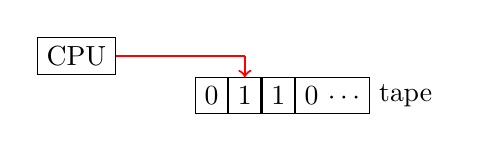
\begin{tikzpicture}[ampersand replacement=\&]
\matrix 
{
  \node[draw](0) {CPU}; \& [1cm] \& \node(1){}; \&\&\& \\
  \& \node[draw]{0}; \& \node[draw](a){1}; \& \node[draw]{1}; \& \node[draw]{0 $\cdots$};  \& \node{tape};\\
};
\draw [-,red,thick] (0) -- (1.center) ;
\draw [->,red,thick] (1.center) -- (a) ;
\end{tikzpicture}
\end{center}


\item Differences from finite automata
  \begin{itemize}
  \item write/read tape
  \item head moves left/right
  \item infinite space in the tape
  \item rejecting/accepting take immediate effect

  \item machine goes on forever, otherwise
  \end{itemize}
\item Example

  \begin{equation*}
B=\{w\#w\mid w \in \{0.1\}^*\}
\end{equation*}
\item This language is known to be not a CFL (example 2.22; details
  not discussed)

\item Running a sample input. Figure 3.2
\item $\sqcup$: blank symbol
\item [] We assume infinite $\sqcup$'s after the input sequence
\item Strategy: zig-zag to the corresponding places on the two sides of the \# and determine
  whether they match.
  
\begin{center}
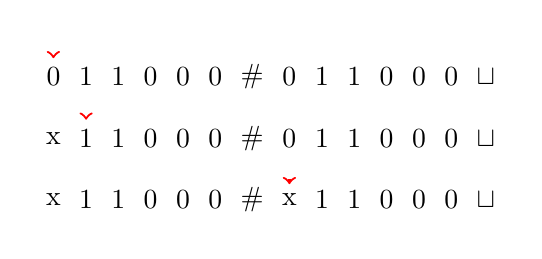
\begin{tikzpicture}[ampersand replacement=\&]
\matrix 
{
  \node(0){};  \&\&\&\&\&\& \& \&\&\&\&\&\& \\
  \node(01){0}; \& \node{1}; \& \node{1}; \& \node{0}; \& \node{0}; \&\node{0}; \&
  \node{\#}; \& 
  \node{0}; \& \node{1}; \& \node{1}; \& \node{0}; \& \node{0}; \& \node{0}; \& \node{$\sqcup$}; \\
    \& \node(1){};  \&\&\&\&\& \& \&\&\&\&\&\& \\
  \node{x}; \& \node(11){1}; \& \node{1}; \& \node{0}; \& \node{0}; \&\node{0}; \&
  \node{\#}; \& 
  \node{0}; \& \node{1}; \& \node{1}; \& \node{0}; \& \node{0}; \& \node{0}; \& \node{$\sqcup$}; \\
\&\&\&\&\&\& \&    \node(2){};   \&\&\&\&\&\& \\
  \node{x}; \& \node{1}; \& \node{1}; \& \node{0}; \& \node{0}; \&\node{0}; \&
  \node{\#}; \& 
  \node(21){x}; \& \node{1}; \& \node{1}; \& \node{0}; \& \node{0}; \& \node{0}; \& \node{$\sqcup$}; \\
};
\draw [->,red,thick] (0) -- (01) ;
\draw [->,red,thick] (1) -- (11) ;
 \draw [->,red,thick] (2) -- (21) ;
% \draw [->,red,thick] (1.center) -- (a) ;
\end{tikzpicture}
\end{center}



\item Algorithm:
  \begin{enumerate}
  \item scan to check \#
  \item check $w$ and $w$
  \end{enumerate}

\end{itemize}
\end{frame}

\begin{frame}[allowframebreaks] \frametitle{Formal definition of TM}
  \begin{itemize}
\item It's complicated and seldom used
\item $\delta$:
  \begin{equation*}
  Q\times \Gamma\rightarrow 
Q\times \Gamma \times\{L,R\}
\end{equation*}
\item Example:
  \begin{equation*}
  \delta(q,a) = (r,b,L)
\end{equation*}
\item [] $q$: current state

\item [] $a$: pointed in tape

\item [] $r$: next state

\item [] $b$: replace $a$ with $b$
\item $(Q,\Sigma, \Gamma, \delta, q_0, q_{accept},
q_{reject})$

\item [] $Q$: states

\item [] $\Sigma$: input alphabet (blank: $\sqcup \notin \Sigma$)

\item [] $\Gamma$: tape alphabet, $\sqcup \in \Gamma, 
\Sigma \subset \Gamma$

\item [] $\delta$:
  \begin{equation*}
  Q\times \Gamma \rightarrow
Q \times \Gamma \times 
\{L,R\}
\end{equation*}
\item [] $q_0 \in Q$, start

\item [] $q_{accept} \in Q$

\item [] $q_{reject} \in Q, q_{reject} \neq q_{accept}$

\item [] Single $q_{accept}, q_{reject}$

\item The input
  \begin{equation*}
  w_1\cdots w_n
\end{equation*}
is put in 
  positions $1 \ldots, n$ of the tape in the beginning

\item [] Assume $\sqcup$ in all the rest of the tape
  
\end{itemize}\end{frame}

\begin{frame}[allowframebreaks] \frametitle{Example 3.7}
  \begin{itemize}
\item Consider the following language
  \begin{equation*}
\{0^{2^n}\mid n \geq 0\}
\end{equation*}
Strings in this language are
\begin{equation*}
0,00,0000,00000000, \ldots
\end{equation*}
\item Idea: crossing off every other 0 and the remaining string should
  still have even length
\item Example:
  \begin{eqnarray*}
&& 0\underline{0} 0\underline{0}\\
&& 0\underline{0}\\
&& 0
  \end{eqnarray*}
\item Procedure
  \begin{enumerate}
  \item left $\rightarrow$ right, mark every other 0
  \item if in step 1, only one 0 left, then accept
  \item if in step 1, odd \# 0 left, then reject
\item move head to the beginning
\item go back to stage 1
  \end{enumerate}

\item Formally definition

\item [] $Q=\{q_1, q_2, q_3, q_4, q_5, q_{accept}, q_{reject}\}$

\item [] $\Sigma=
  \{0\}$

\item[] $\Gamma=\{0, x, \sqcup\}$
\item The diagram
\end{itemize}
\begin{tikzpicture}
\node[state,initial above] (q_1) {$q_1$};
\node[state] (q_2) [right of=q_1,xshift=0.5cm] {$q_2$};
\node[state] (q_3) [right of=q_2,xshift=1.7cm] {$q_3$};
\node[state] (q_4) [below of=q_3, yshift=0cm, xshift=0cm] {$q_4$};
\node[state] (q_5) [above right of=q_2, yshift=0cm] {$q_5$};
\node[state] (q_r) [below of=q_1, yshift=0cm] {$q_r$};
\node[state] (q_a) [below of=q_2, yshift=0.7cm] {$q_a$};
 \path 
 (q_1) edge[below]  node {$0 \rightarrow \sqcup$, R} (q_2)
 (q_1) edge[right]  node {
   \begin{tabular}{l}
     $\sqcup \rightarrow$ R\\
     x   $ \rightarrow$ R\\
   \end{tabular}} (q_r)
 (q_2) edge[loop above]  node {x $ \rightarrow $ R} (q_2)
 (q_2) edge[below]  node {$0 \rightarrow $ x, R} (q_3)
 (q_2) edge[right]  node {$\sqcup \rightarrow $ R} (q_a) 
 (q_3) edge[left, bend right=15]  node {$0 \rightarrow $ R} (q_4)
 (q_3) edge[loop right]  node {x $ \rightarrow $ R} (q_3)
 (q_3) edge[right]  node {$\sqcup \rightarrow $ L} (q_5) 
 (q_4) edge[right, bend right=15]  node {$0 \rightarrow $ x, R} (q_3)
 (q_4) edge[loop left]  node {x $ \rightarrow $ R} (q_4)
 (q_4) edge[above, bend left=20]  node {$\sqcup \rightarrow $ R} (q_r)
 (q_5) edge[loop right]  node {
   \begin{tabular}{l}
     $0 \rightarrow $ L\\
     x $\rightarrow$ L
   \end{tabular}
 } (q_5)
 (q_5) edge[right]  node {$\sqcup \rightarrow$ R } (q_2)    
;
  \end{tikzpicture}
\begin{itemize}

\item $0 \rightarrow R\equiv 0 \rightarrow 0, R$

\item Consider the input 0000
  \begin{center}
  \begin{tabular}{lllll}
    $q_1 0000$ & $\sqcup q_2 000$ & $\sqcup x q_3 00$ & $\sqcup x 0 q_4 0$
    & $\sqcup x 0 x q_3$                                         \\
    $\sqcup x 0 q_5 x$ & $\sqcup x q_5 0 x$ & $\sqcup q_5 x 0 x$
    &  $q_5 \sqcup x 0 x$ & $\sqcup q_2  x 0 x$ \\
$\sqcup x q_2  0 x$ & $\sqcup x x q_3  x$ & $\sqcup x x x q_3  \sqcup $
& $\sqcup x x q_5 x $ & $\sqcup x q_5 x x $\\
$\sqcup q_5 x x x $ & $q_5 \sqcup  x x x $ & $\sqcup  q_2 x x x $
& $\sqcup  x q_2 x x $ & $\sqcup  x x q_2 x $ \\
$\sqcup  x x x q_2$ & $\sqcup  x x x \sqcup q_a$ &&&
  \end{tabular}
\end{center}
\item  The $\delta$ function:

  \begin{center}
\begin{tabular}{c|ccc}
& 0 & x & $\sqcup$\\ \hline
$q_1 $ & $q_2,\sqcup,R$ & $q_{reject},x,R$ & $q_{reject},\sqcup,
R$\\
$q_2$ & $q_3,x,R$ & $q_2,x,R$ & $q_{accept},\sqcup,R$
\end{tabular}
\end{center}

\item No need to have rows for $q_{accept},q_{reject}$

\item [] $\Rightarrow$ accepting/rejecting takes immediate effect

\item Now a deterministic TM

\item [] We can have nondeterministic TM later

\item [] They are equivalent

\item Main idea of $\delta$:

\item $q_1: $ mark the start by
$\sqcup$
\begin{itemize}
\item first element must be 0, otherwise, reject
\item Using $\sqcup$, so the start is known
\end{itemize}
\item $q_2 \rightarrow q_3$: handle initial 00

\item $q_3\rightarrow q_4$: sequentially $00 \rightarrow 0x$

  \begin{itemize}
  \item key of this algorithm
  \item If not pairs (e.g. 0x0x0x), fails
  \item The place where \# is even checked
  \end{itemize}
$q_3 \rightarrow q_5 \rightarrow q_2 $ back to beginning

% \item Why $q_2, q_3$ cannot be combined

% \item [] $q_3$ sees $\sqcup$: moves left

% \item [] $q_2$ sees $\sqcup$: first $\sqcup$ stop

\item First 0 (or $\sqcup$) is considered the single
final 0 
\begin{equation*}
q_2 \rightarrow \cdots
\rightarrow q_2 \rightarrow \cdots \rightarrow
q_{accept}
\end{equation*}
check if single 0
% \item Exercise 

% 000000

% Even fewer steps than 0000

\end{itemize}\end{frame}


\end{document}
